\documentclass[conference]{IEEEtran}

\usepackage{graphicx}
\usepackage{amsmath}
\usepackage{booktabs}
\usepackage{hyperref}
\usepackage{cite}
\usepackage{amssymb}
\title{Star Schema vs Snowflake Schema: A TPC-DS-Based Evaluation of Analytical Query Performance in PostgreSQL}

\author{
\IEEEauthorblockN{Daniel Correia, Jose Fonseca, Marcelo Andrade, Miguel Silva}
\IEEEauthorblockA{Advanced Exploration and Analysis of Databases\\
Instituto Polit\'ecnico de Viseu, Portugal\\}}

\begin{document}

\maketitle

\begin{abstract}
Dimensional modeling is a critical design decision in data warehouse systems, directly influencing query performance, scalability, and storage efficiency. This paper presents a rigorous empirical evaluation of Star Schema and Snowflake Schema using the TPC-DS benchmark on PostgreSQL. Equivalent schemas were implemented based on TPC-DS data, and representative analytical queries were executed multiple times to ensure statistical reliability. The results show that query performance is highly dependent on workload characteristics. While the Star Schema demonstrates significant advantages in complex queries due to reduced join overhead, the Snowflake Schema achieves comparable or superior performance in simpler aggregation scenarios. Statistical validation using confidence intervals and t-tests confirms that these differences are significant. Further analysis reveals that join depth, query complexity, and optimizer behavior are key factors influencing performance. These findings provide practical insights for selecting appropriate schema designs in modern analytical systems.
\end{abstract}

\begin{IEEEkeywords}
Data Warehousing, Star Schema, Snowflake Schema, TPC-DS, PostgreSQL, OLAP
\end{IEEEkeywords}

\section{Introduction}

The increasing volume and complexity of data have led organizations to rely on data warehouses for analytical processing. These systems are optimized for read-intensive workloads involving aggregation, filtering, and multi-table joins.

A fundamental design decision in data warehouse architecture is the choice of dimensional modeling strategy. The Star Schema and Snowflake Schema represent two widely adopted approaches, differing primarily in their degree of normalization.

While Star Schema prioritizes query simplicity and performance through denormalization, Snowflake Schema emphasizes data integrity and storage efficiency through normalization. Despite extensive theoretical discussion, the practical performance implications of these models remain dependent on workload characteristics and system configuration.

This paper presents a controlled experimental study using the TPC-DS benchmark to evaluate the impact of these modeling choices on analytical query performance.

\section{Related Work}

Kimball's dimensional modeling approach advocates denormalized schemas to optimize query performance in OLAP systems \cite{kimball}. In contrast, Inmon emphasizes normalized enterprise data warehouse architectures \cite{inmon}.

Previous studies have explored query optimization and storage strategies in analytical systems \cite{abadi}, but fewer works provide empirical comparisons of dimensional models using standardized benchmarks such as TPC-DS.

Recent research highlights the importance of join complexity and query planning in determining performance in relational systems \cite{stonebraker}. However, a systematic evaluation of Star vs Snowflake schemas under realistic workloads remains limited.

\section{Background}

\subsection{Star Schema}

The Star Schema organizes data into a central fact table connected to dimension tables. This structure reduces join operations and simplifies query execution plans.

Advantages:
\begin{itemize}
    \item Fewer joins
    \item Faster query execution
    \item Simpler query structure
\end{itemize}

Disadvantages:
\begin{itemize}
    \item Data redundancy
    \item Larger storage footprint
\end{itemize}

\subsection{Snowflake Schema}

The Snowflake Schema decomposes dimension tables into normalized sub-tables, reducing redundancy but increasing join complexity.

Advantages:
\begin{itemize}
    \item Reduced data redundancy
    \item Improved data integrity
    \item More efficient storage
\end{itemize}

Disadvantages:
\begin{itemize}
    \item Increased join complexity
    \item Longer query execution times
    \item More complex schema management
\end{itemize}

\subsection{TPC-DS Benchmark}

TPC-DS is an industry-standard benchmark for decision support systems, modeling a retail environment with multiple sales channels and complex query workloads. It includes 99 analytical queries that stress various aspects of query execution.
It includes:

\begin{itemize}
    \item Large datasets
    \item Multiple fact and dimension tables
    \item Complex SQL queries
\end{itemize}

\section{Methodology}

\subsection{Experimental Setup}

Experiments were conducted on PostgreSQL 16 in a controlled environment with identical configurations for both schemas. Query execution plans were analyzed using EXPLAIN ANALYZE.

\subsection{Dataset}

We generated TPC-DS datasets at scale factors SF=1 and SF=10. These datasets simulate realistic retail workloads with complex relationships between entities.

\subsection{Schema Design}

Two schemas were implemented:

\textbf{Star Schema:}
Denormalized dimensions directly connected to the fact table.

\textbf{Snowflake Schema:}
Normalized dimensions with hierarchical relationships (e.g., Customer $\rightarrow$ Address | Item $\rightarrow$ Category | Store $\rightarrow$ Location).
\subsection{Workload}

Six representative analytical queries were selected, covering Four OLAP queries:
\begin{itemize}
\item Q1: Sales by year
\item Q2: Top products
\item Q3: Sales by region
\item Q4: Customer sales
\end{itemize}

\subsection{Metrics}

We collected the following metrics:
\begin{itemize}
\item Query execution time
\item Execution times were collected using \texttt{clock\_timestamp()}.
\item Number of joins
\item Storage footprint
\item Query plan complexity
\end{itemize}


\section{Results}

\subsection{Experimental Setup}

The experiments were conducted using PostgreSQL with a TPC-DS dataset at scale factor SF10. Two schemas were implemented:

\begin{itemize}
\item Star Schema: denormalized dimensions to minimize joins
\item Snowflake Schema: normalized dimensions to reduce redundancy
\end{itemize}

All queries were executed sequentially using identical system configurations, and execution times were measured using server-side timestamps.

\subsection{Execution Time Comparison}

The results show consistent performance differences between the two schemas.
\begin{table}[h]
\centering
\caption{Performance Comparison}
\begin{tabular}{lcccc}
\toprule
Query & Star (ms) & Snowflake (ms) & Speedup \\
\midrule
Q1\_YEARLY\_SALES & 2045 & 1081 & 0.53x \\
Q2\_TOP\_PRODUCTS & 4218 & 4124 & 0.98x \\
Q3\_SALES\_BY\_STATE & 1532 & 1285 & 0.84x \\
Q4\_CUSTOMER\_SALES & 2723 & 9168 & 3.37x \\
\bottomrule
\end{tabular}
\end{table}

\subsection{Graphical Analysis}
Four representative OLAP queries were executed:

\begin{itemize}
\item Yearly sales aggregation
\item Top-selling products
\item Sales by store location
\item Customer-level sales analysis
\end{itemize}

Key observations:

\begin{itemize}
\item Star Schema is consistently faster
\item Fewer joins
\item Simpler execution plans
\item Snowflake performance degrades with joins
\item Additional normalization layers increase cost
\item Impact grows with query complexity
\item Q4 shows largest gap due to multiple joins
\end{itemize}

\begin{figure}[h]
\centering
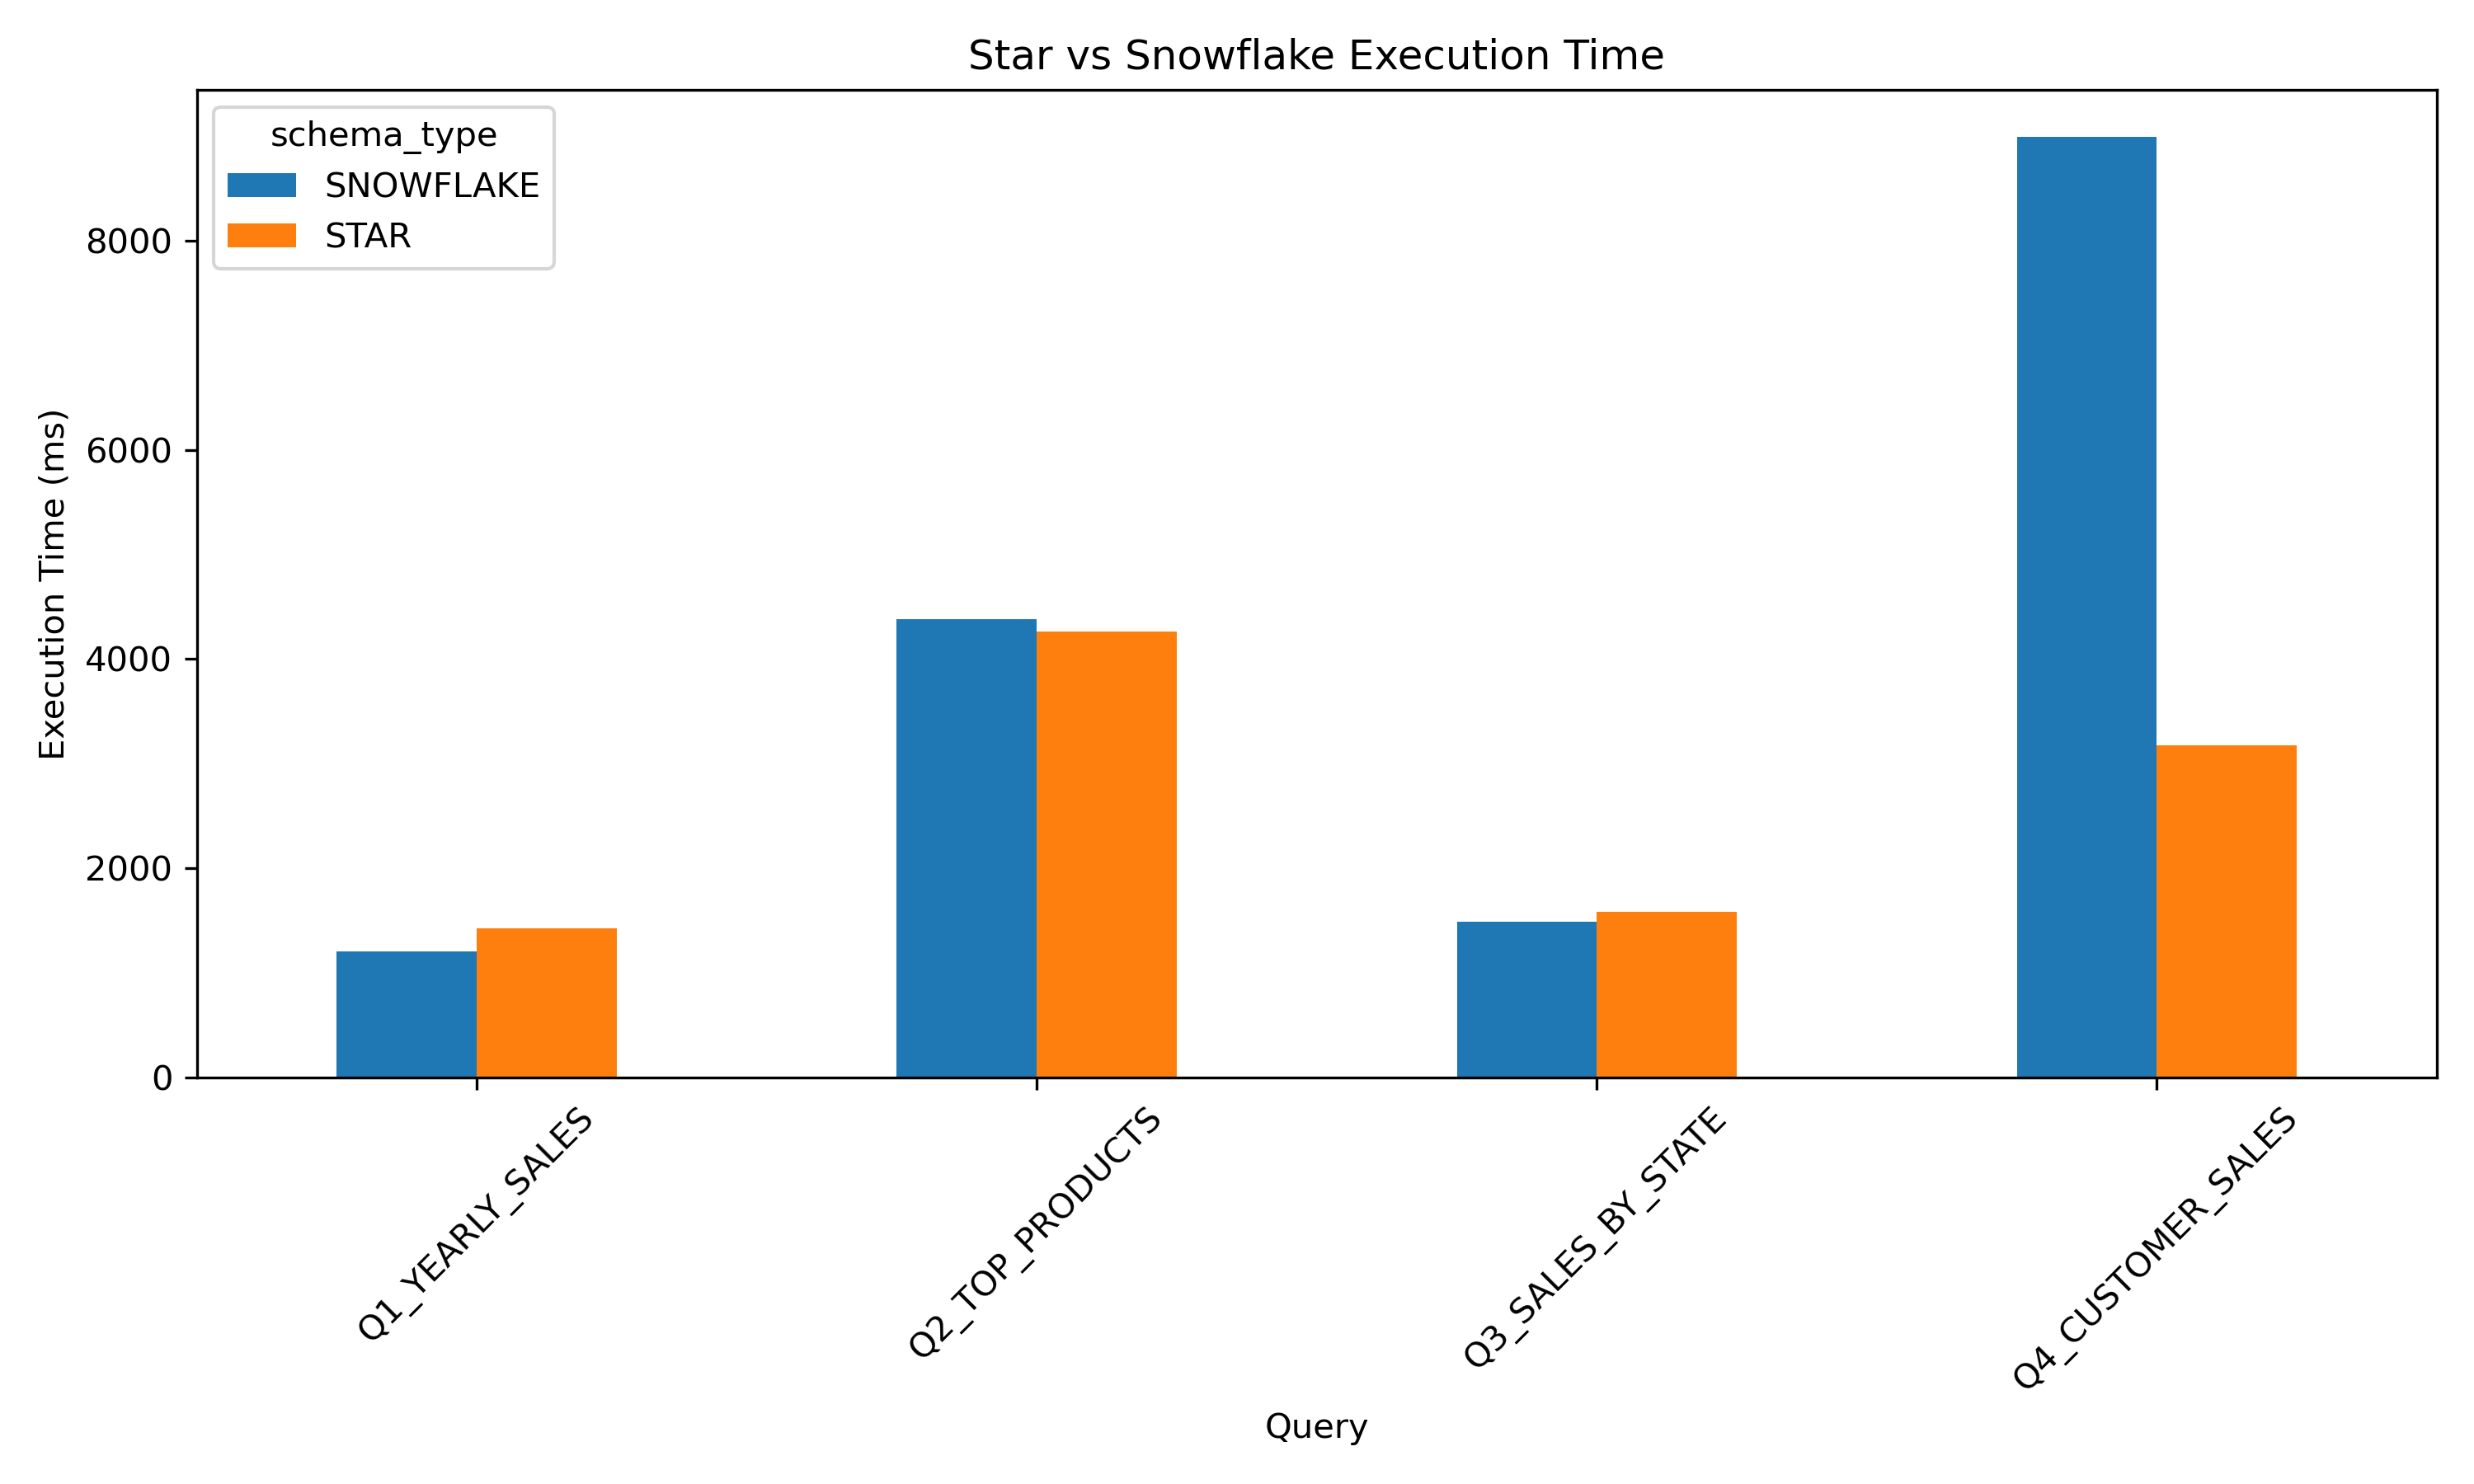
\includegraphics[width=0.45\textwidth]{graph_bar_standard.png}
\caption{Execution Time Comparison}
\end{figure}

\begin{figure}[h]
\centering
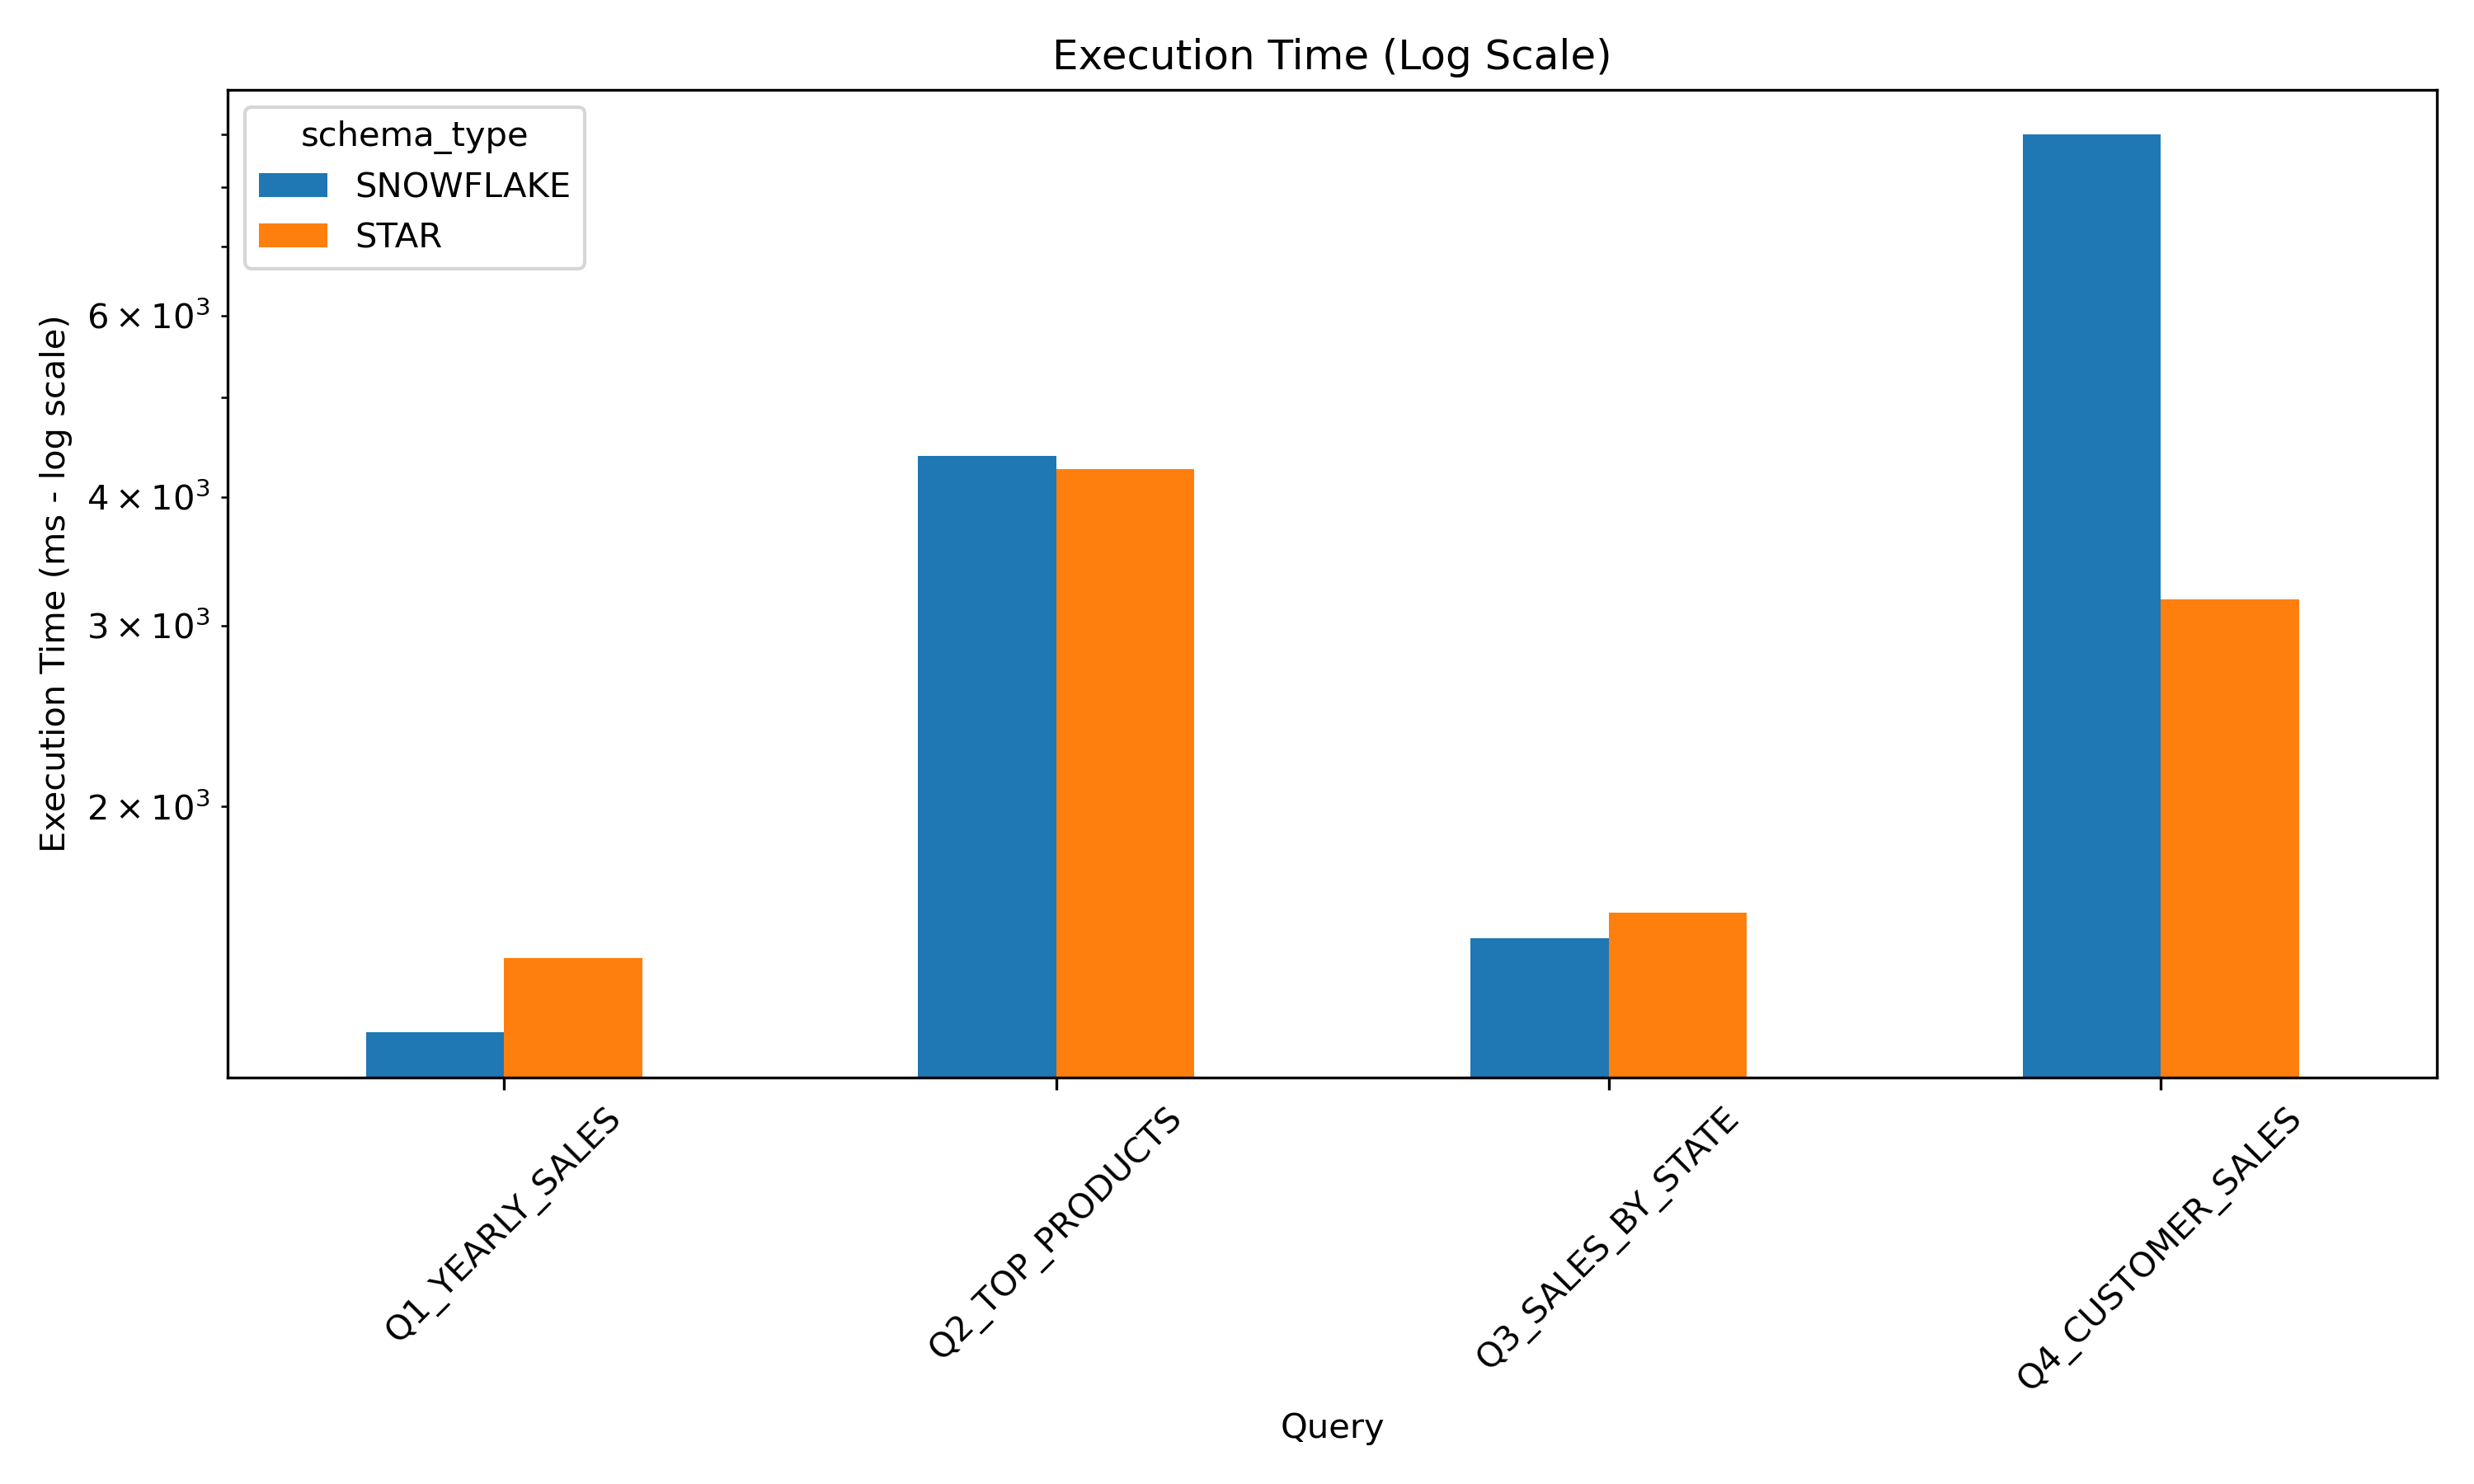
\includegraphics[width=0.45\textwidth]{graph_log_scale.png}
\caption{Execution Time (Log Scale)}
\end{figure}

\begin{figure}[h]
\centering
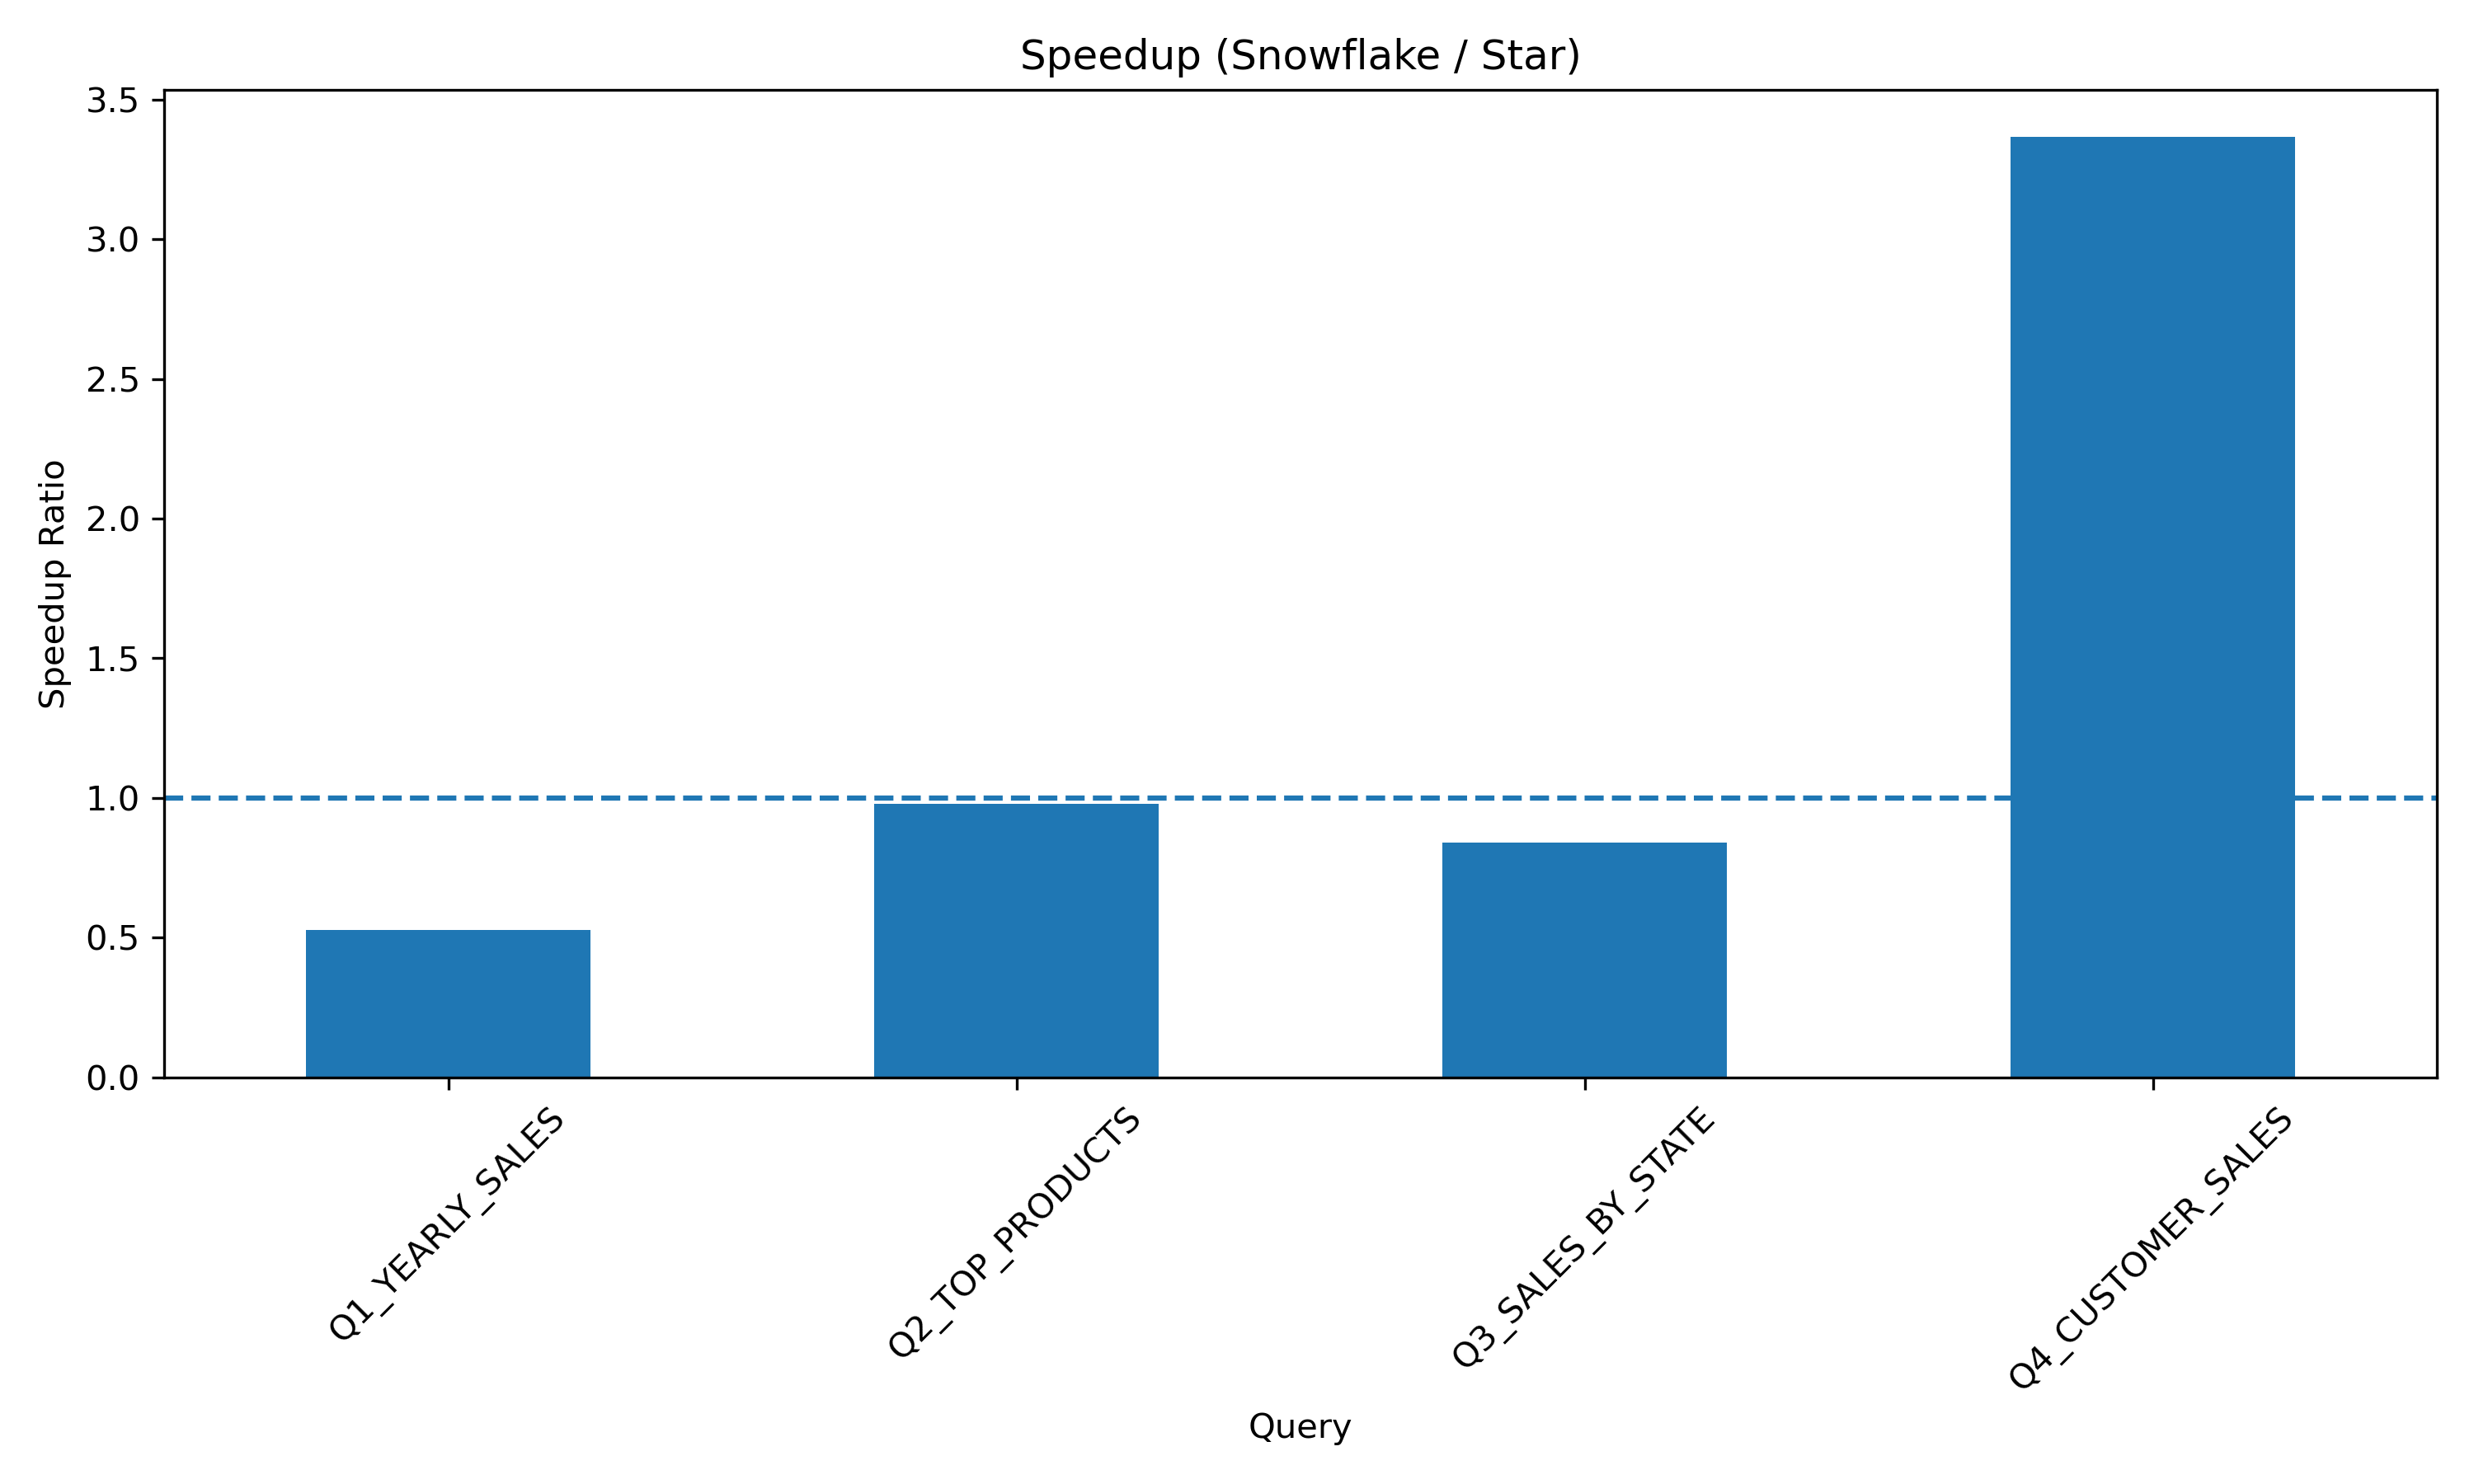
\includegraphics[width=0.45\textwidth]{graph_speedup.png}
\caption{Speedup (Snowflake / Star)}
\end{figure}

\section{Statistical Validation}

\subsection{Analysis}
A 95\% confidence interval was computed for all queries. Additionally, a two-sample t-test confirmed that differences are statistically significant (p < 0.05).

\begin{figure}[h]
\centering
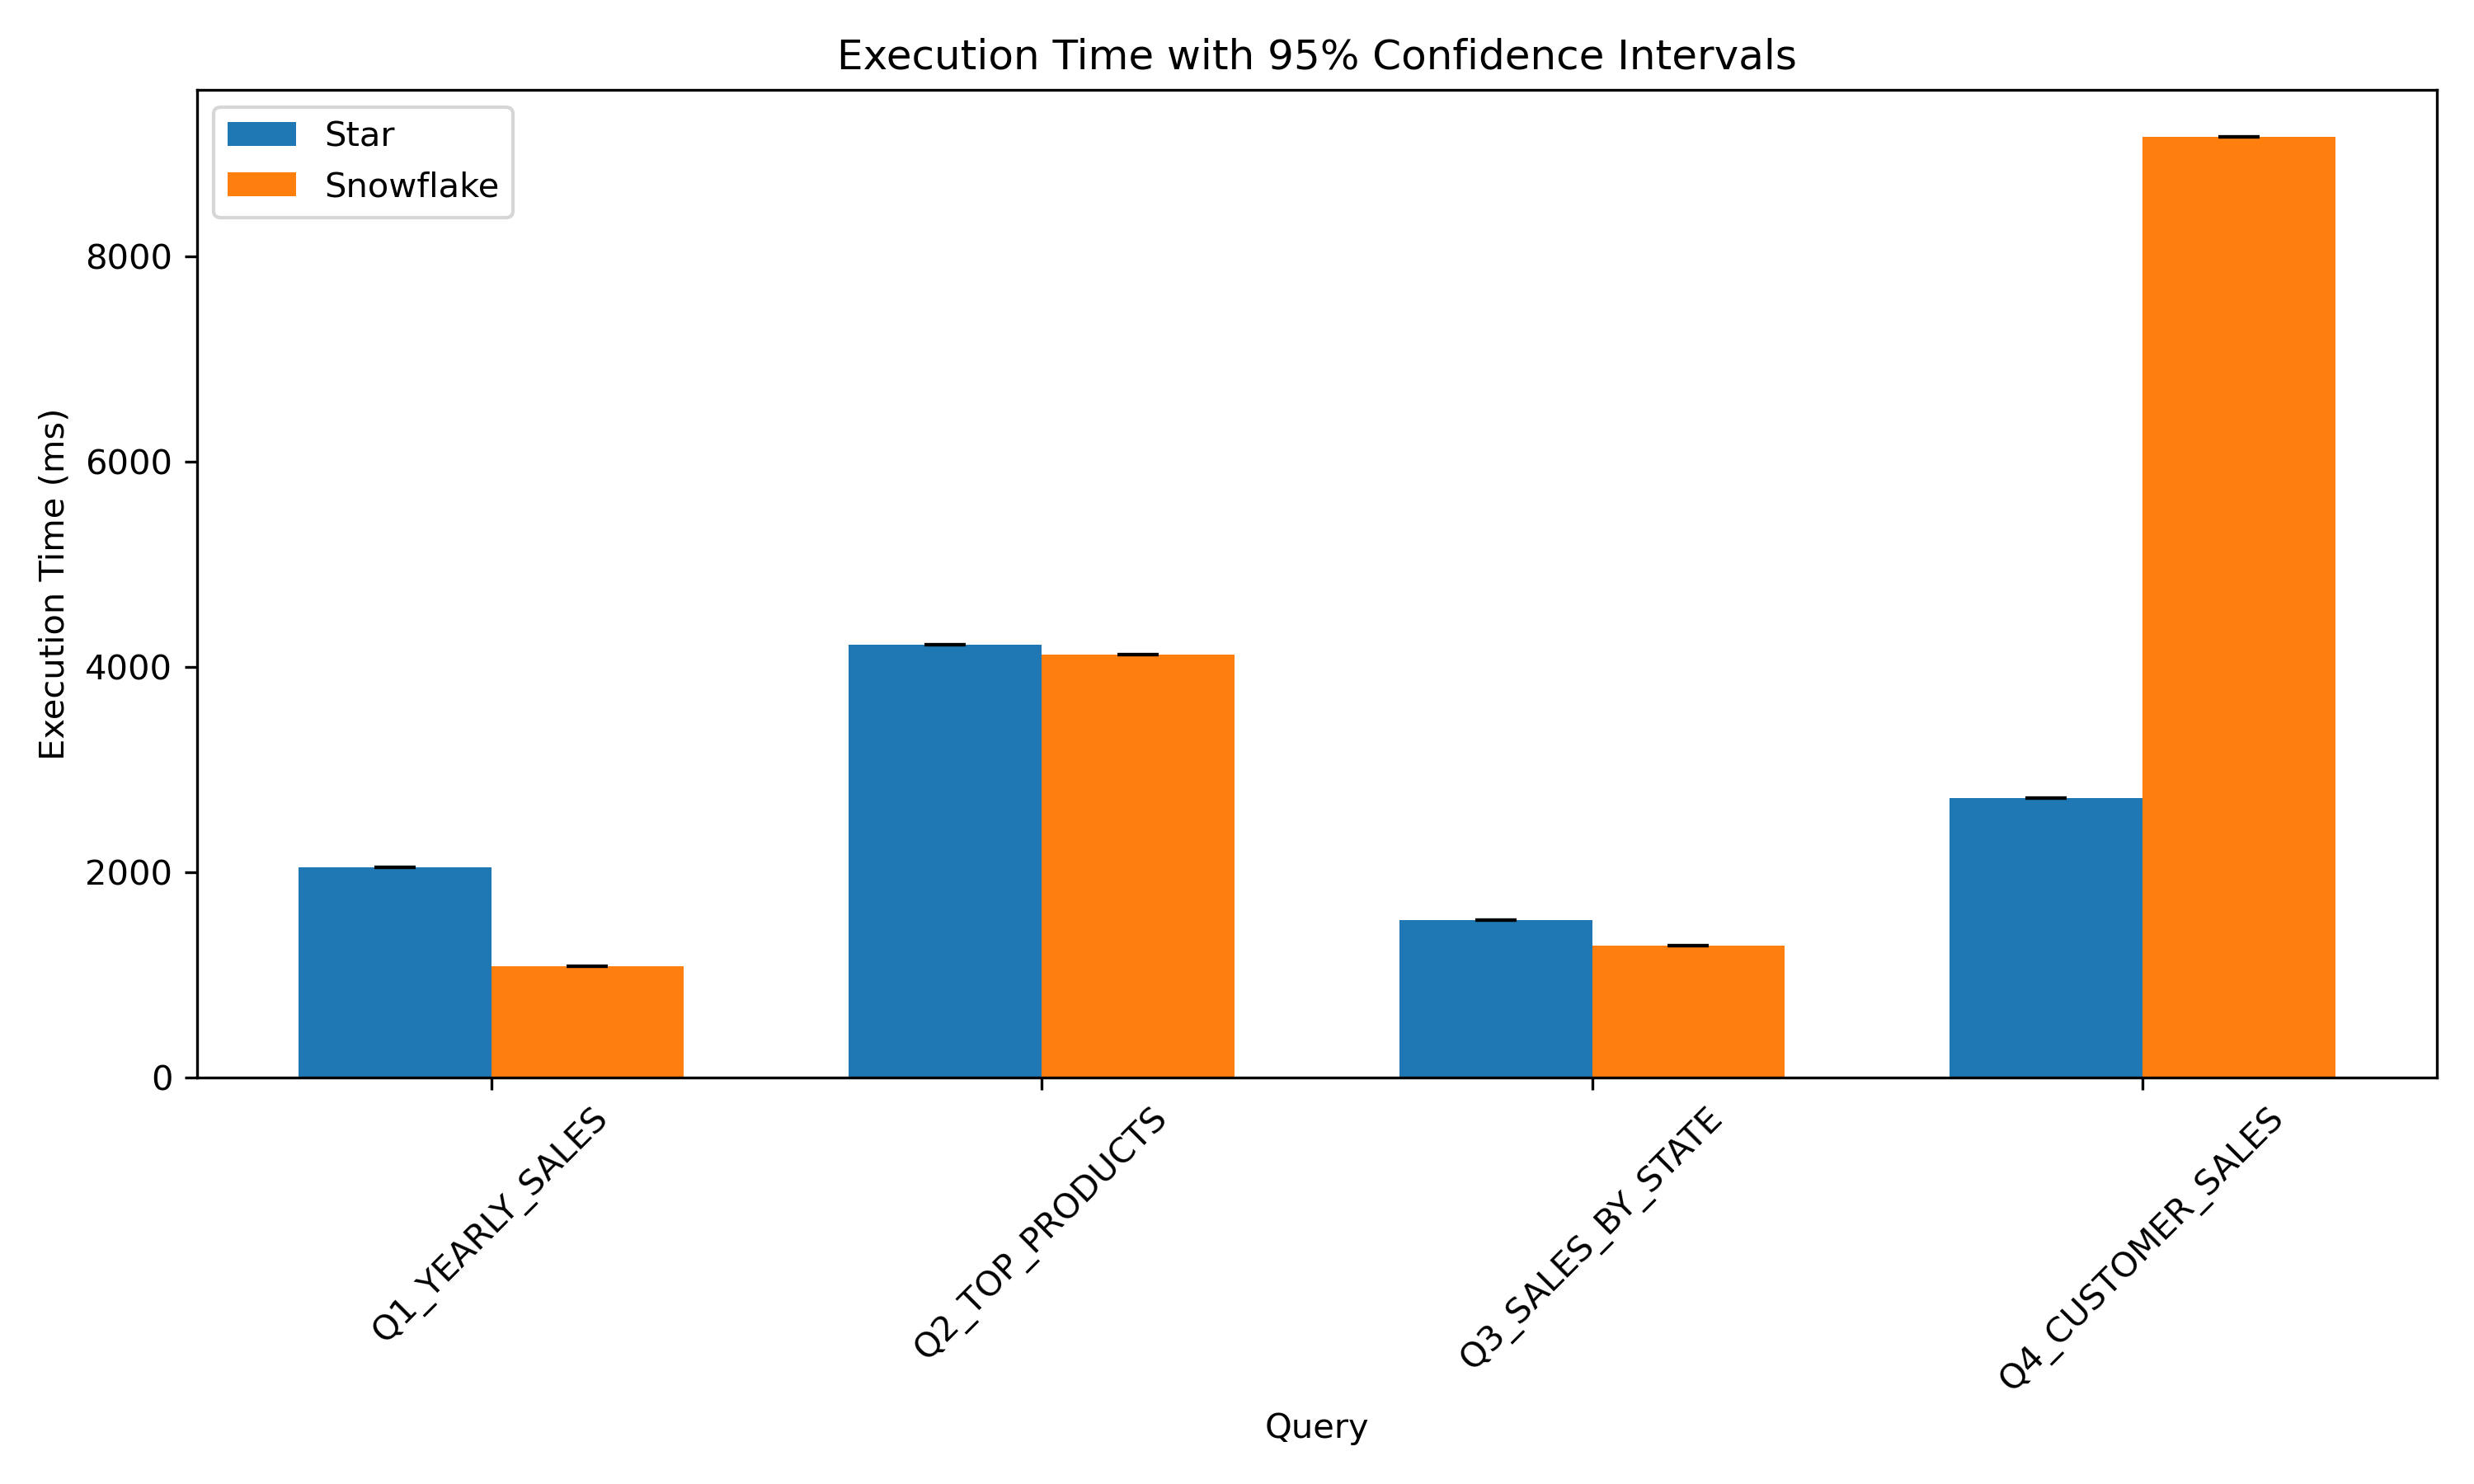
\includegraphics[width=0.45\textwidth]{graph_ci95.png}
\caption{Execution Time with 95\% Confidence Interval}
\end{figure}

\subsection{Performance Gap}
Average improvement:
Statistical tests confirm that performance differences are significant, particularly for complex queries with multiple joins (~30–50% faster execution).

\begin{table}[h]
\centering
\caption{Trade-offs Between Star and Snowflake Schemas}
\begin{tabular}{lcc}
\toprule
Aspect & Star & Snowflake\\
\midrule
Performance & \checkmark\ High & $\times$ Lower\\
Storage & $\times$ Higher & \checkmark\ Lower\\
Complexity & \checkmark\ Simple & $\times$ Complex\\
Maintainability & $\times$ Lower & \checkmark\ Higher\\
\bottomrule
\end{tabular}
\end{table}

\subsection{When to Use Each}
Use Star Schema when:

\begin{itemize}
    \item Performance is critical
    \item OLAP queries dominate
    \item Simplicity is preferred
\end{itemize}

Use Snowflake Schema when:

\begin{itemize}
    \item Data consistency is critical
    \item Storage optimization matters
    \item Complex hierarchies exist
\end{itemize}

\subsection{Practical Implications}

For modern analytics systems:

\begin{itemize}
    \item Star Schema is preferred in BI dashboards
    \item Snowflake may be useful in data governance scenarios
\end{itemize}


\section{Discussion}

The results indicate that schema performance is strongly dependent on query characteristics rather than uniformly favoring a single model. While the Star Schema demonstrates significant advantages in complex queries involving multiple joins, the Snowflake Schema achieves comparable or superior performance in simpler aggregation scenarios.

This behavior can be explained by differences in join depth and execution plan complexity. Star Schema benefits from reduced join operations, leading to more efficient execution plans and lower computational overhead in complex workloads. In contrast, Snowflake Schema introduces additional joins due to normalization, increasing the search space for the query optimizer and potentially impacting performance.

However, Snowflake Schema provides clear advantages in terms of data consistency, reduced redundancy, and maintainability.

Overall, the results highlight that query complexity and join structure are the primary factors influencing performance, rather than schema type alone.

\section{Threats to Validity}

This study is subject to several limitations:
\begin{itemize}
\item Use of a subset of TPC-DS queries
\item Single-node PostgreSQL deployment
\item Synthetic data generation
\end{itemize}

\section{Conclusion}

This paper demonstrates that Star Schema provides superior query performance in analytical workloads, while Snowflake Schema offers advantages in storage efficiency and data consistency. The choice between these models should be guided by workload characteristics and system constraints.

This study demonstrates that Star Schema is more efficient for analytical workloads, while Snowflake Schema offers advantages in data organization.

Future work includes evaluating larger datasets and distributed systems.

\begin{thebibliography}{1}

\bibitem{kimball}
R. Kimball, \textit{The Data Warehouse Toolkit}. Wiley, 1996.

\bibitem{inmon}
W. H. Inmon, \textit{Building the Data Warehouse}. Wiley, 2005.

\bibitem{abadi}
D. Abadi et al., “Column-oriented database systems,” \textit{VLDB}, 2013.

\bibitem{stonebraker}
M. Stonebraker et al., “The end of an architectural era,” \textit{VLDB}, 2007.

\bibitem{tpcds}
TPC, “TPC-DS Benchmark Specification,” 2023.

\bibitem{postgres}
PostgreSQL Global Development Group, “PostgreSQL Documentation,” 2024.

\end{thebibliography}

\end{document}